% %% %%%%%%%%%%%%%%%%%%%%%%%%%%%%%%%%%%%%%%%%%%%%%%%%%%%%%%%%%%
% intro-triac.tex
%
% Author:  Mauricio Matamoros
% License: MIT
%
% %% %%%%%%%%%%%%%%%%%%%%%%%%%%%%%%%%%%%%%%%%%%%%%%%%%%%%%%%%%%
%!TEX root = ../practica.tex
%!TEX root = ../references.bib

% CHKTEX-FILE 1
% CHKTEX-FILE 13
% CHKTEX-FILE 46

\subsection{TRIACs}%
\label{seq:intro-triac}

Un TRIAC o triodo interruptor para corriente alterna (\emph{Triode AC Switch}) es un integrado de estado sólido compuesto por dos tristores conectados en paralelo inverso (véase~\Cref{fig:triac-analogy}) que permite conmutar la corriente que pasa por un circuito de AC a alta frecuencia de manera similar a como operan los transistores bipolares y FETs en DC.
Es decir, un TRIAC es un interruptor de estado sólido que puede operar a gran velocidad que, a diferencia de los relés, no existe la posibilidad de que un arco eléctrico funda los metales y el dispositivo se quede en encendido permanente, sino que al quemarse un TRIAC siempre abre el circuito.
Por otro lado, basta una corriente muy pequeña entre el gate ($G$) y cualquiera de las terminales ($MT_1$ y $MT_2$) para encender al TRIAC, lo que lo convierte en el aliado ideal para controlar dispositivos de alta potencia con un microcontrolador.

\begin{figure}[H]
	\centering
	\begin{subfigure}{0.3\linewidth}
		\centering
		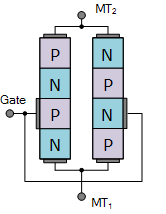
\includegraphics{img/triac1.png}
		\caption{Construcción física}%
		\label{fig:triac-construction}
	\end{subfigure}
	\begin{subfigure}{0.3\linewidth}
		\centering
		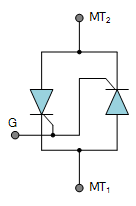
\includegraphics{img/triac2.png}
		\caption{Equivalente en tristores}%
		\label{fig:triac-analogy}
	\end{subfigure}
	\begin{subfigure}{0.3\linewidth}
		\centering
		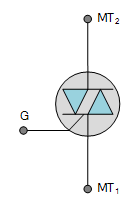
\includegraphics{img/triac3.png}
		\caption{Símbolo}%
		\label{fig:triac-symbol}
	\end{subfigure}
	\caption[Triac]{El Triac\footnotemark{}}%
		\label{fig:triac}
\end{figure}
\footnotetext{Fuente de imagen: \url{https://www.electronics-tutorials.ws/power/triac.html}}

Como siempre, al utilizar un TRIAC es deseable aislar la parte de corriente directa del circuito de la parte de corriente alterna, es decir, el TRIAC deberá estar aislado pero acoplado al circuito DC.
Esto normalmente se realiza mediante el uso de optoacopladores tipo MOC, tal como se ilustra en la \Cref{fig:triac-circuit}.

\begin{figure}[H]
	\centering
	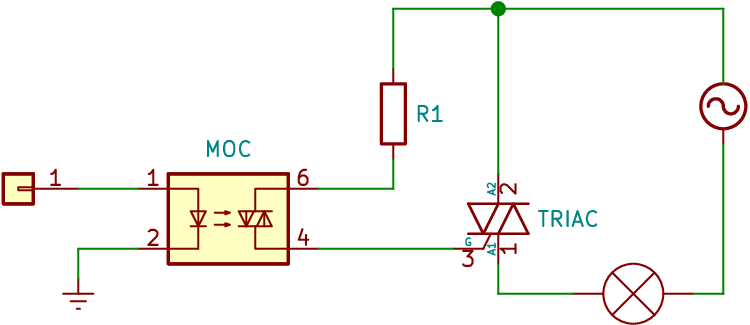
\includegraphics[width=0.5\textwidth,height=5cm,keepaspectratio]{img/triac-circuit.png}
	\caption{Triac optoacoplado}
	\label{fig:triac-circuit} %chktex 24
\end{figure}
